%& /home/nidish/.cache/org-persist/64/e51324-6d1b-45a5-aa1b-4951960488e0-a1f9df0debad2cb0170443c4dd6918a2
% Created 2026-10-16 Fri 17:54
% Intended LaTeX compiler: pdflatex
\documentclass[11pt]{article}
\usepackage[utf8]{inputenc}
\usepackage[T1]{fontenc}
\usepackage{amsmath}
\usepackage{amssymb}
\usepackage{capt-of}
\usepackage{hyperref}
\usepackage{graphicx}
\usepackage{wrapfig}
\usepackage{rotating}
\usepackage{longtable}
\usepackage[margin=1in]{geometry}
\usepackage[subrefformat=parens,labelformat=parens]{subcaption}
\usepackage{siunitx}
\usepackage{xcolor}
\usepackage{accents}
\usepackage{minted}
\usepackage{cancel}
\newcommand{\vc}[1]{\underbar{$#1$}}
\newcommand{\mx}[1]{\mathbf{\underline{\underbar{$#1$}}}\,}
\newcommand{\uc}[1]{\underaccent{\tilde}{#1}}
\newcommand{\mc}[1]{\underaccent{\approx}{#1}}
\usepackage{cleveref}

%% ox-latex features:
%   !announce-start, !guess-pollyglossia, !guess-babel, !guess-inputenc,
%   caption, image, !announce-end.

\usepackage{capt-of}

\usepackage{graphicx}

%% end ox-latex features


% end precompiled preamble
\ifcsname endofdump\endcsname\endofdump\fi

\author{Nidish Narayanaa Balaji}
\date{October 16, 2026}
\title{SDynPy WorkBench\\\medskip
\large Example Usage}
\hypersetup{
 pdfauthor={Nidish Narayanaa Balaji},
 pdftitle={SDynPy WorkBench},
 pdfkeywords={},
 pdfsubject={},
 pdfcreator={},
 pdflang={English}}
\begin{document}

\maketitle
\tableofcontents

\section*{Introduction}
\label{sec:org9988ab4}
This is an example usage of the GUI workbench built on top of \href{https://sandialabs.github.io/sdynpy/}{SDynPy}. We employ modal testing data from an impact hammer based modal test conducted on a metallic bowl (2 sensors and 8 impact locations) in tandem with a finite element model of the same prepared using \href{https://open-simulation-center.org/fr/downloads/code\_aster/SALOME\_MECA}{Salome$\backslash$\textsubscript{Meca}} (solver: Code$\backslash$\textsubscript{Aster}). We employ the finite element mode shapes to expand the experimental mode shapes through the System Equivalent Reduction Expansion Process (SEREP) implemented in SDynPy post the modal fitting.
\section{Launch the Workbench}
\label{sec:orge03f63f}
\begin{verbatim}
python3 sdynpy_workbench.py 
\end{verbatim}

\begin{figure}[!h]
\centering
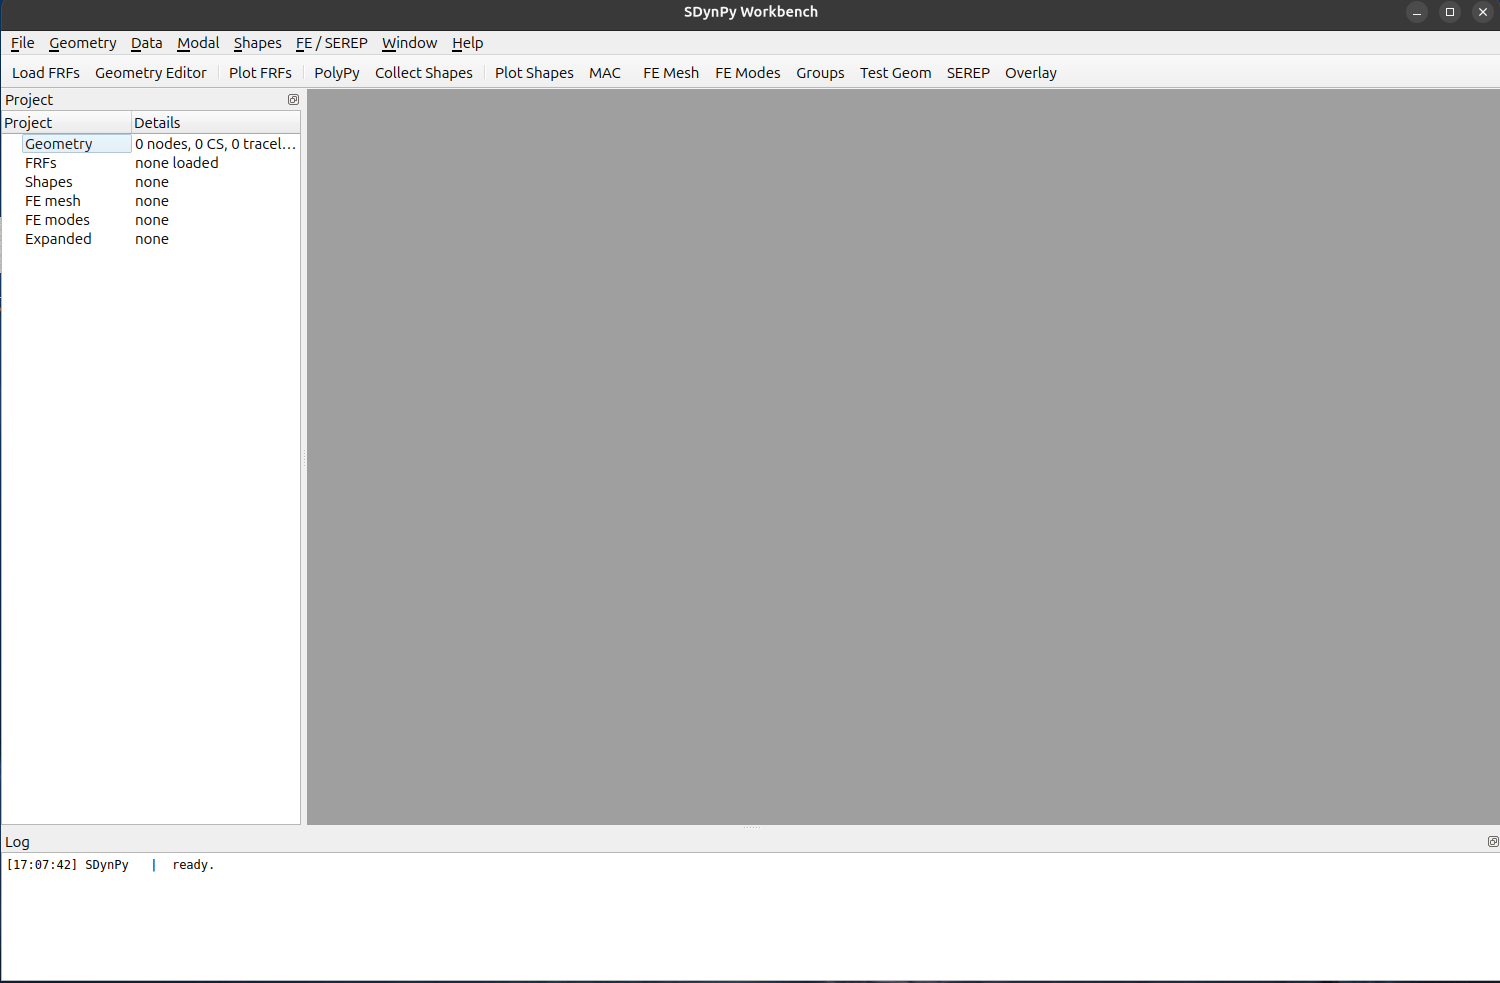
\includegraphics[width=0.75\linewidth]{figs/wb1.png}
\caption{\label{fig:wb1}The Launching Screen for the Workbench}
\end{figure}

\Cref{fig:wb1} shows the landing screen of the GUI. There are several ways to "get started" from here, you may choose to use one some of these. 
\begin{itemize}
\item \textbf{You can load the measured FRFs} with the \texttt{Load FRFs} button and then go on to \texttt{Plot FRFs} and also \texttt{PolyPy} for the modal fitting. This will allow you to do the modal fitting but it is not possible to plot mode shapes or anything since no geometry was created. The modal analysis is based on the \href{https://sandialabs.github.io/sdynpy/sdynpy-polypy-gui/}{PolyPy GUI} implemented in SDynPy. While loading, the workbench gives you an option of "symmetrizing" the measurements - this is sometimes helpful when measured data is noisy and does not obey reciprocity strictly.

\item \textbf{You can manually create the test geometry} with \texttt{Geometry Editor} which allows you to type in nodal locations, define coordinates, and also define tracelines and elements. This is fully based on the \href{https://sandialabs.github.io/sdynpy/geometry/}{Geometry edit GUI} implemented in SDynPy.

Once both the above are done, it will be possible to visualize mode-shapes through PolyPy.
\end{itemize}
\section{Load Geometry from an FE Mesh.}
\label{sec:org4bb13b1}

We shall now load the geometry from an FE mesh and also define local coordinate systems at the sensor attachment locations. We can do this by:
\begin{enumerate}
\item Click on \texttt{FE Mesh} and load up the MED file that has the mesh. We also have a node set which has the sensor locations of our test. In our example the "results" file \texttt{resu.rmed} stores the mesh also so this is loaded.

\begin{figure}[!h]
\centering
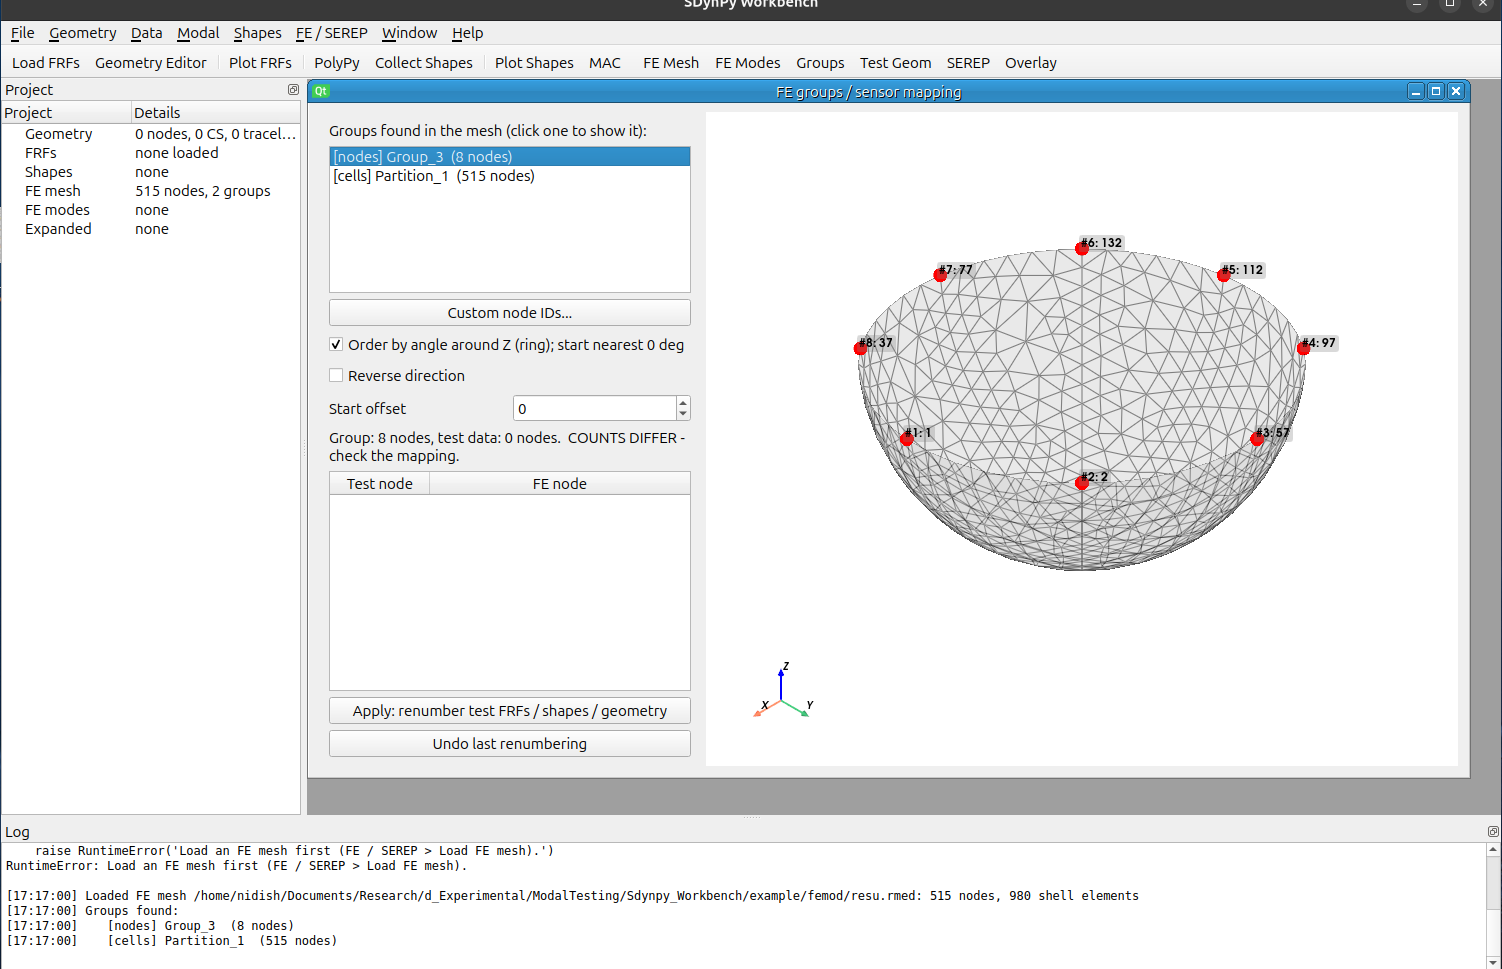
\includegraphics[width=0.75\textwidth]{figs/femesh.png}
\caption{\label{fig:femesh}GUI state after FE mesh is loaded}
\end{figure}

\Cref{fig:femesh} shows the GUI state where the "Group\textsubscript{3}" group has the relevant nodes.

\item Click on \texttt{Test Geom} 

Now we shall create a test geometry using a subset of the nodes from the FE mesh coming from the above group. 

\begin{figure}[!h]
\centering
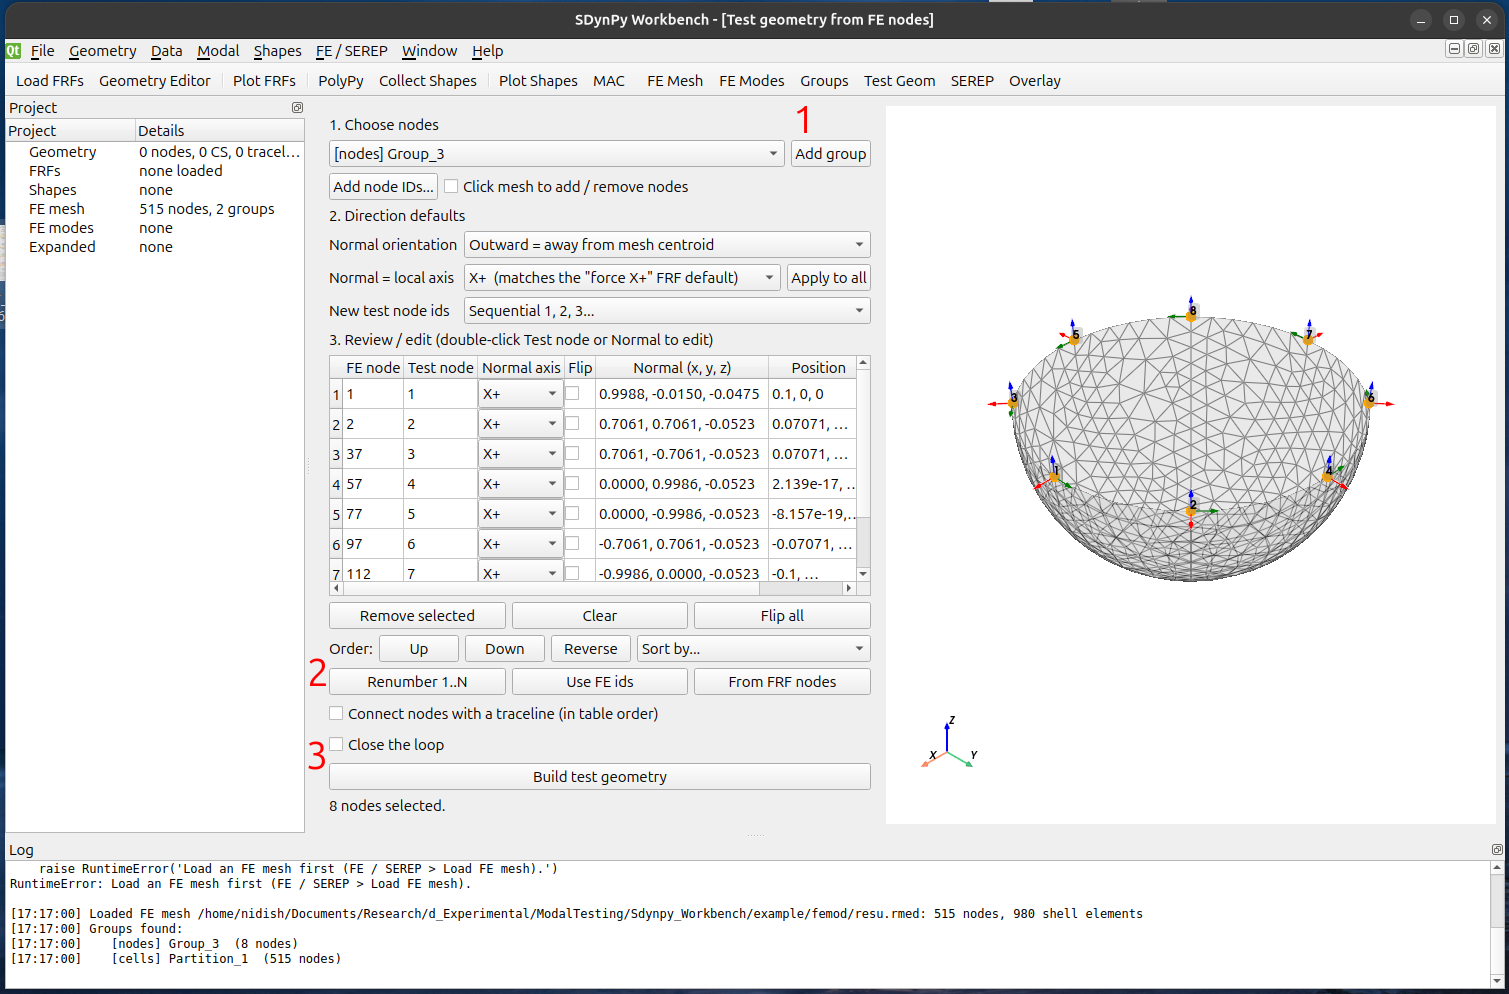
\includegraphics[width=0.75\textwidth]{figs/testgeom.png}
\caption{\label{fig:testgeom}GUI state after \texttt{Test Geom}.}
\end{figure}

\Cref{fig:testgeom} shows the state of the GUI right after \texttt{Test Geom} is clicked.

\begin{enumerate}
\item Firstly (see 1 in figure) we click on "Add group" (also explore the other options) to highlight the relevant group;

\item Then (see 2 in figure) we reorder and renumber the nodes so they match the ordering used in the test;

\item Finally (see 3 in figure) we create the tracelines for visualizations and click on \texttt{Build test geometry}.
\end{enumerate}

After this, clicking on \texttt{Geometry Editor} will show the test geometry that has been created, as shown in \cref{fig:testgeomar} below. We have also selected \texttt{Show DOF Arrows} to demonstrate that local coordinate systems have been appropriately defined.

\begin{figure}[!h]
\centering
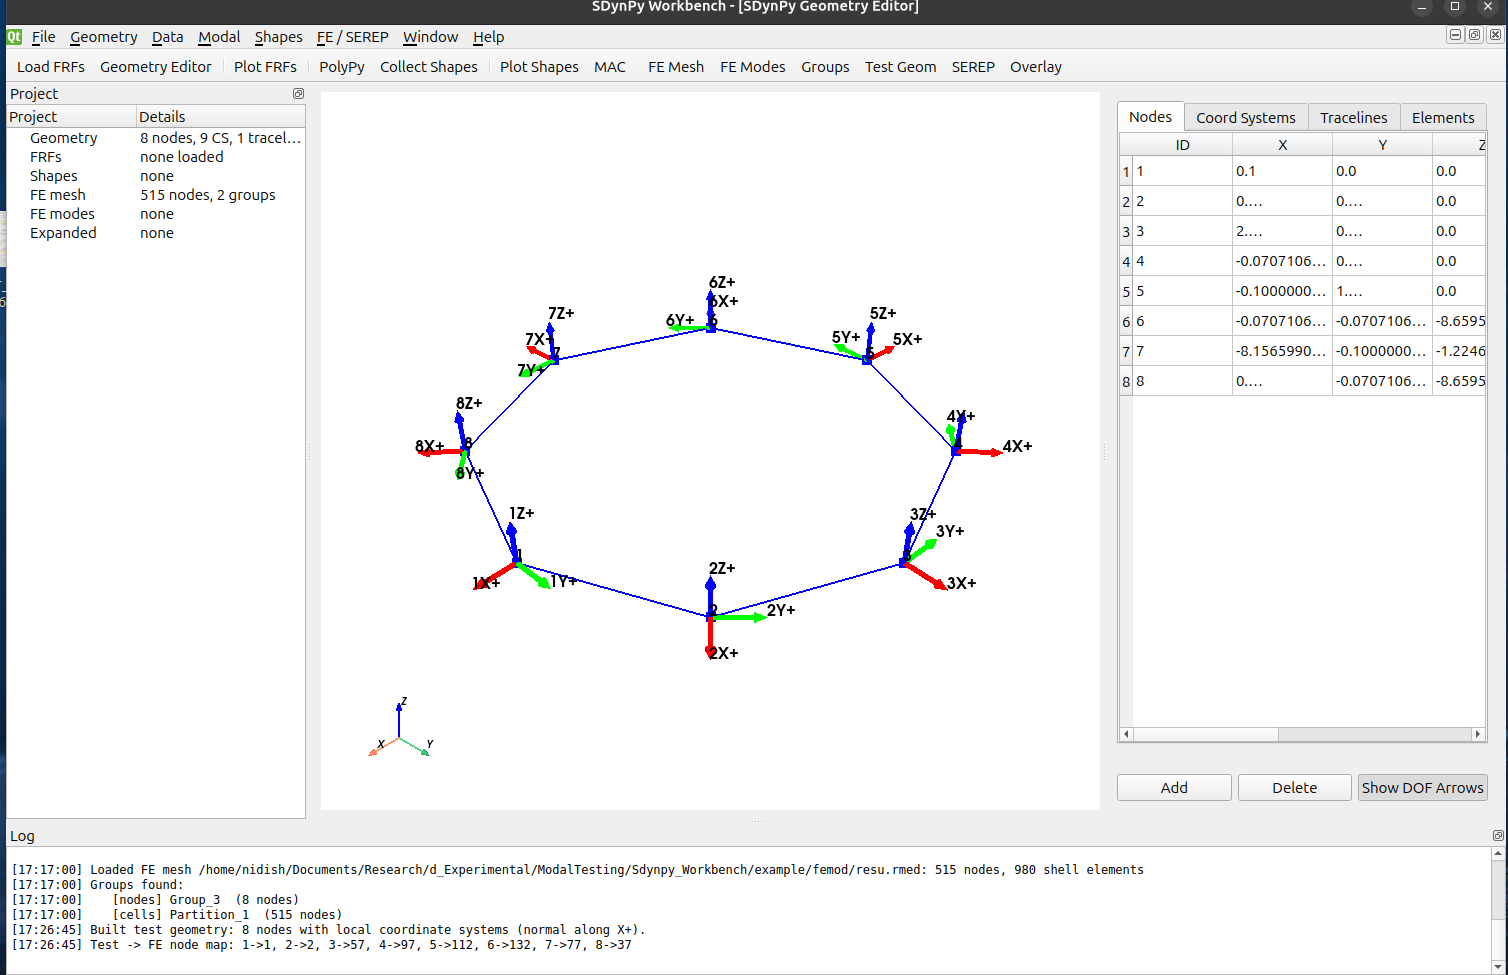
\includegraphics[width=0.75\textwidth]{figs/testgeomar.png}
\caption{\label{fig:testgeomar}The GUI state after \texttt{Geometry Editor} and then \texttt{Show DOF Arrows} are pressed.}
\end{figure}
\end{enumerate}
\section{Conduct the PolyPy modal fitting.}
\label{sec:org00aa2a2}

Now we click on \texttt{PolyPy} to do the modal fitting. Read the SDynPy docs to see more. \Cref{fig:polypy} shows the GUI state at the end of the polypy fitting. 

\begin{figure}[!h]
\centering
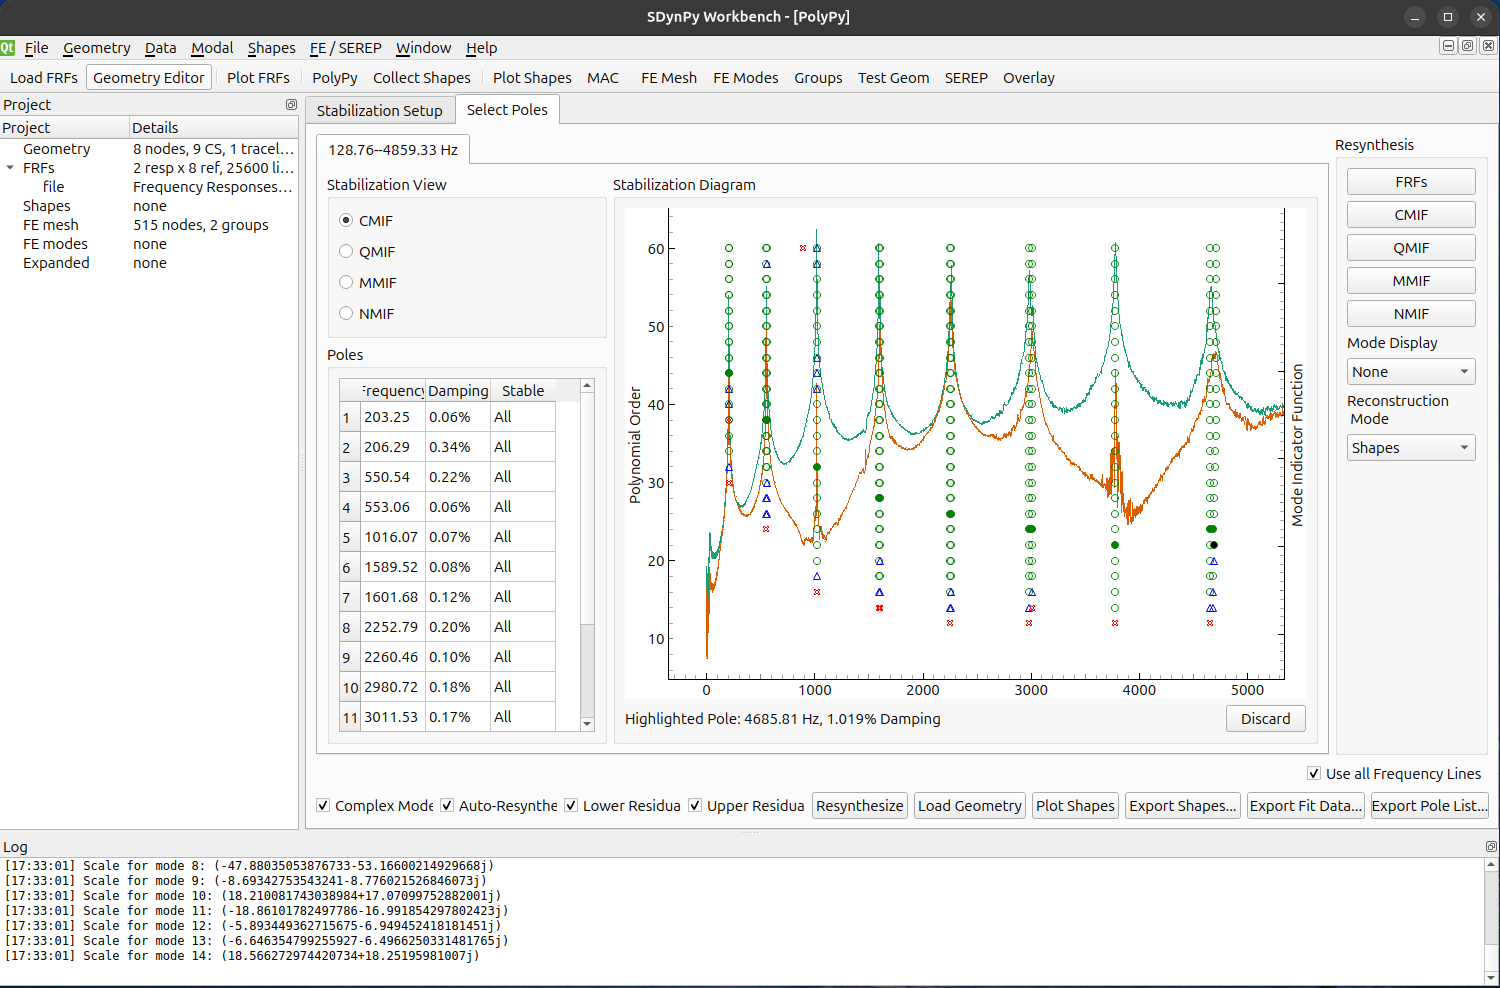
\includegraphics[width=0.75\textwidth]{figs/polypy.png}
\caption{\label{fig:polypy}The GUI state after the end of the PolyPy fitting}
\end{figure}
\section{Visualize the mode shapes on the test geometry.}
\label{sec:orgfca9090}

We can visualize the mode shapes on the test geometry by clicking on \texttt{Plot Shapes} within the PolyPy subwindow. \Cref{fig:testshapes} shows the GUI state that also visualizes the first mode shape on the test geometry.

\begin{figure}[!h]
\centering
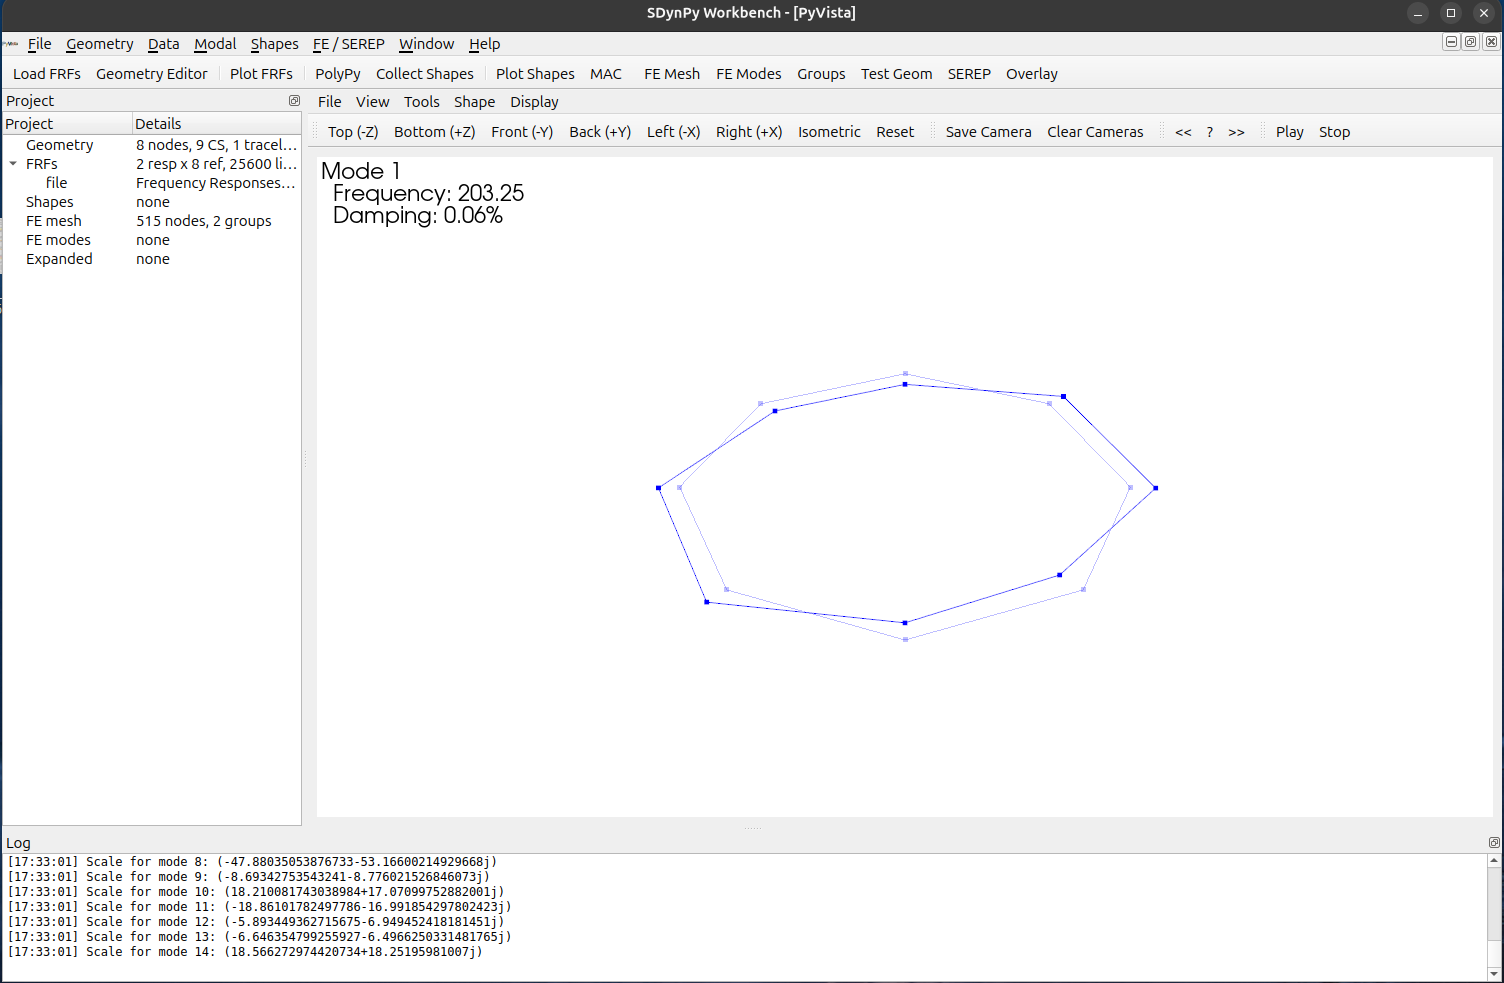
\includegraphics[width=0.75\textwidth]{figs/pshapes.png}
\caption{\label{fig:testshapes}The GUI state after \texttt{Plot Shapes} is clicked}
\end{figure}

We click on \texttt{Collect Shapes} on the top to accept the PolyPy fit. Note that this will be updated on the Project tree in the left. 

Next we shall move on to the \textbf{System Equivalent Reduction Expansion Process (SEREP)} for expanding the test shapes onto the shapes computed through FE. 
\section{Renumber the node indices on the test geometry to match with the FE model}
\label{sec:org210ac85}

Now the node indices on the test geometry do not match the node indices on the FE geometry. So we click on \texttt{Groups} to renumber the test nodes. (\emph{note: you may have to re-load the FE mesh for this})

\begin{figure}[!h]
\centering
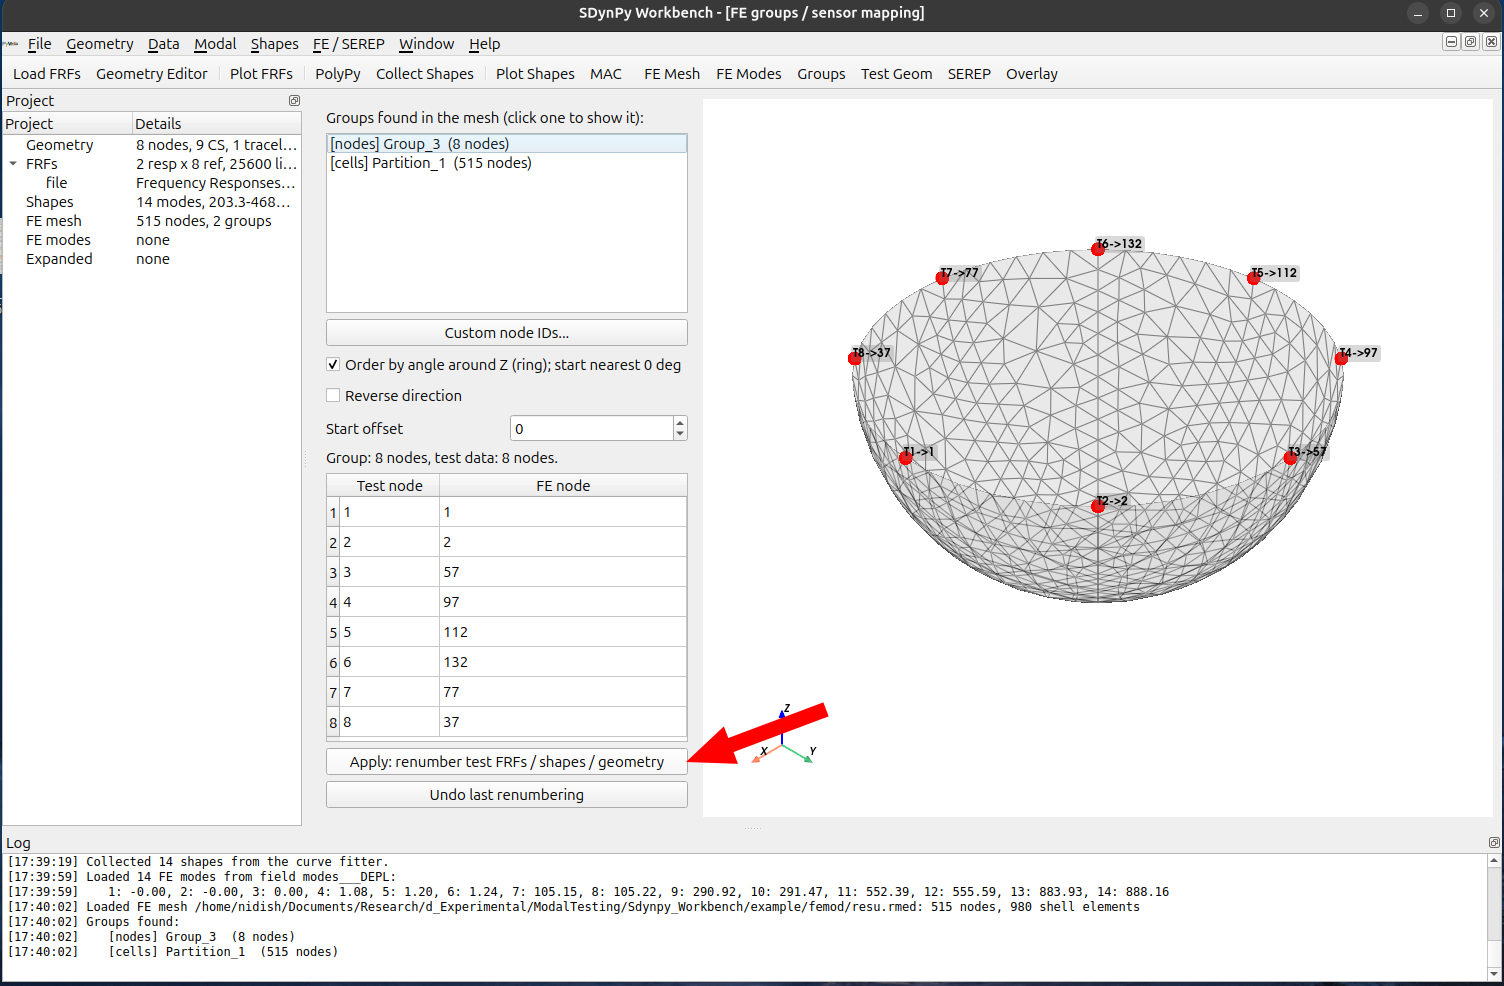
\includegraphics[width=0.75\textwidth]{figs/renum.png}
\caption{\label{fig:renum}GUI state after clicking on \texttt{Groups}}
\end{figure}

\Cref{fig:renum} shows the GUI state after \texttt{Groups} is clicked. Now the table lists the nodes for renumbering - check this and then click on \texttt{Apply:renumber test FRFs/shapes/geometry}.
\section{Load the finite element mode shapes by clicking on \texttt{FE Modes}.}
\label{sec:org37d5be0}

We choose the "resu.rmed" file to load up the FE mode shapes by clicking on \texttt{FE Modes}. After this we may visualize the FE modes by \texttt{FE/SEREP->Plot FE Modes} just to visualize through SDynPy.
\section{Click on the \texttt{SEREP} button to choose the modes to use for the SEREP}
\label{sec:org436d545}

\Cref{fig:serepmodes} shows the pop up that appears after the \texttt{SEREP} button is clicked. We can here choose which modes to use. I shall choose modes 7,8,9,10 and click Ok.

\begin{figure}[!h]
\centering
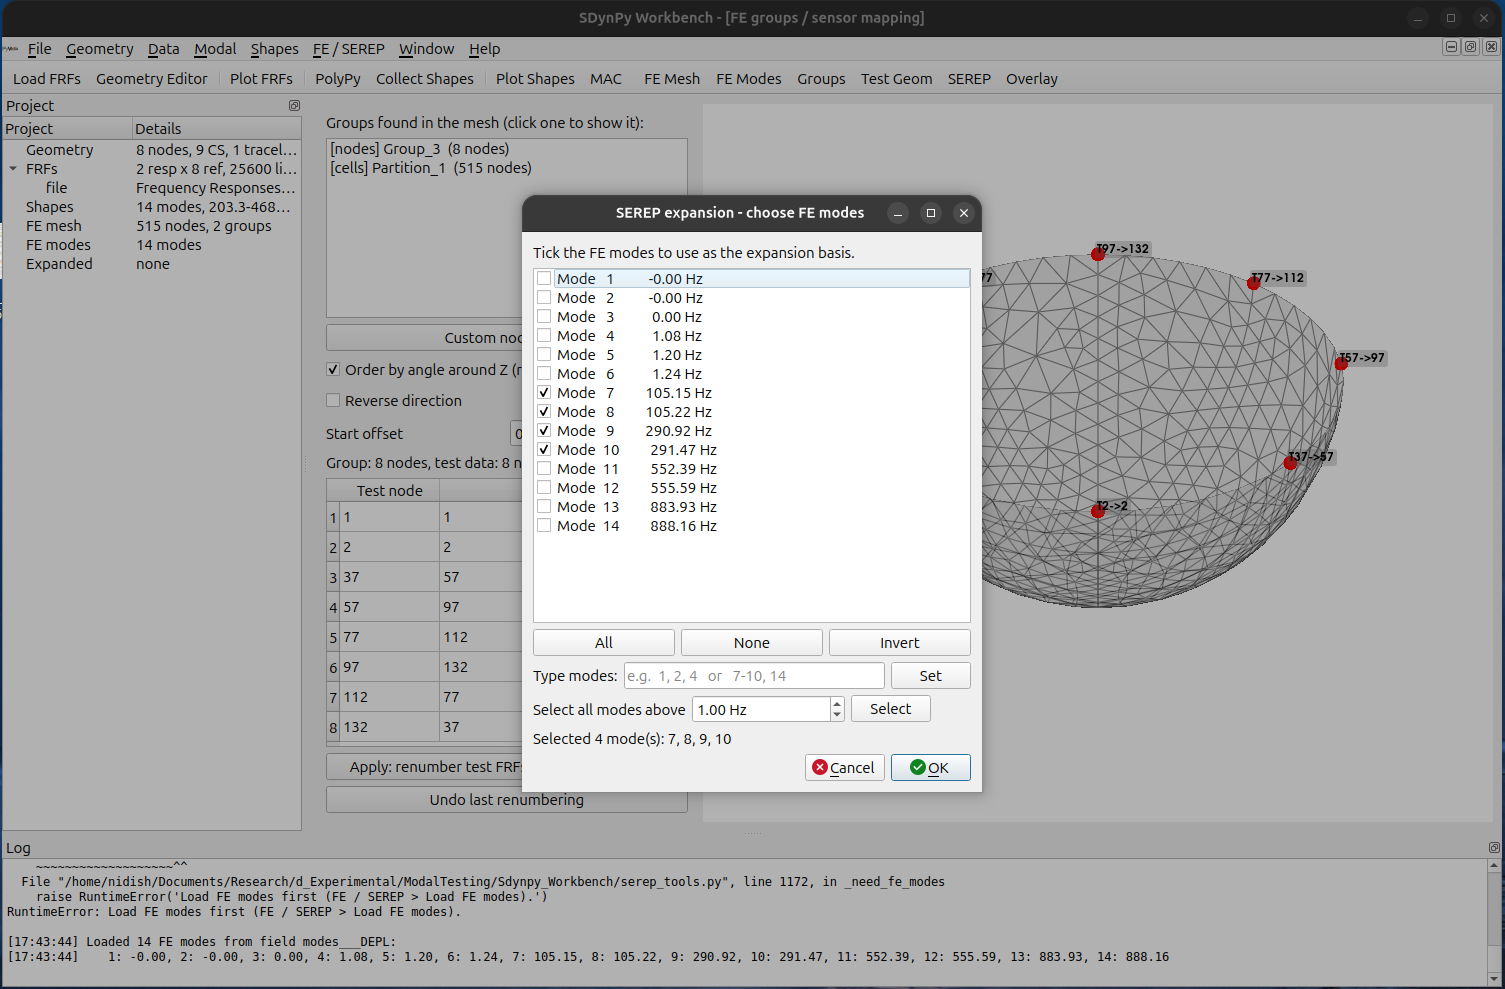
\includegraphics[width=0.75\textwidth]{figs/serepmodes.png}
\caption{\label{fig:serepmodes}GUI state after clicking on \texttt{SEREP}}
\end{figure}

This would conduct the SEREP using the implementation in SDynPy and show the expanded mode shapes. Click on \texttt{Overlay} to visualize the expanded modeshapes along with the test geometry shapes. \Cref{fig:overlay} shows the overlaid modeshape.

\begin{figure}[htbp]
\centering
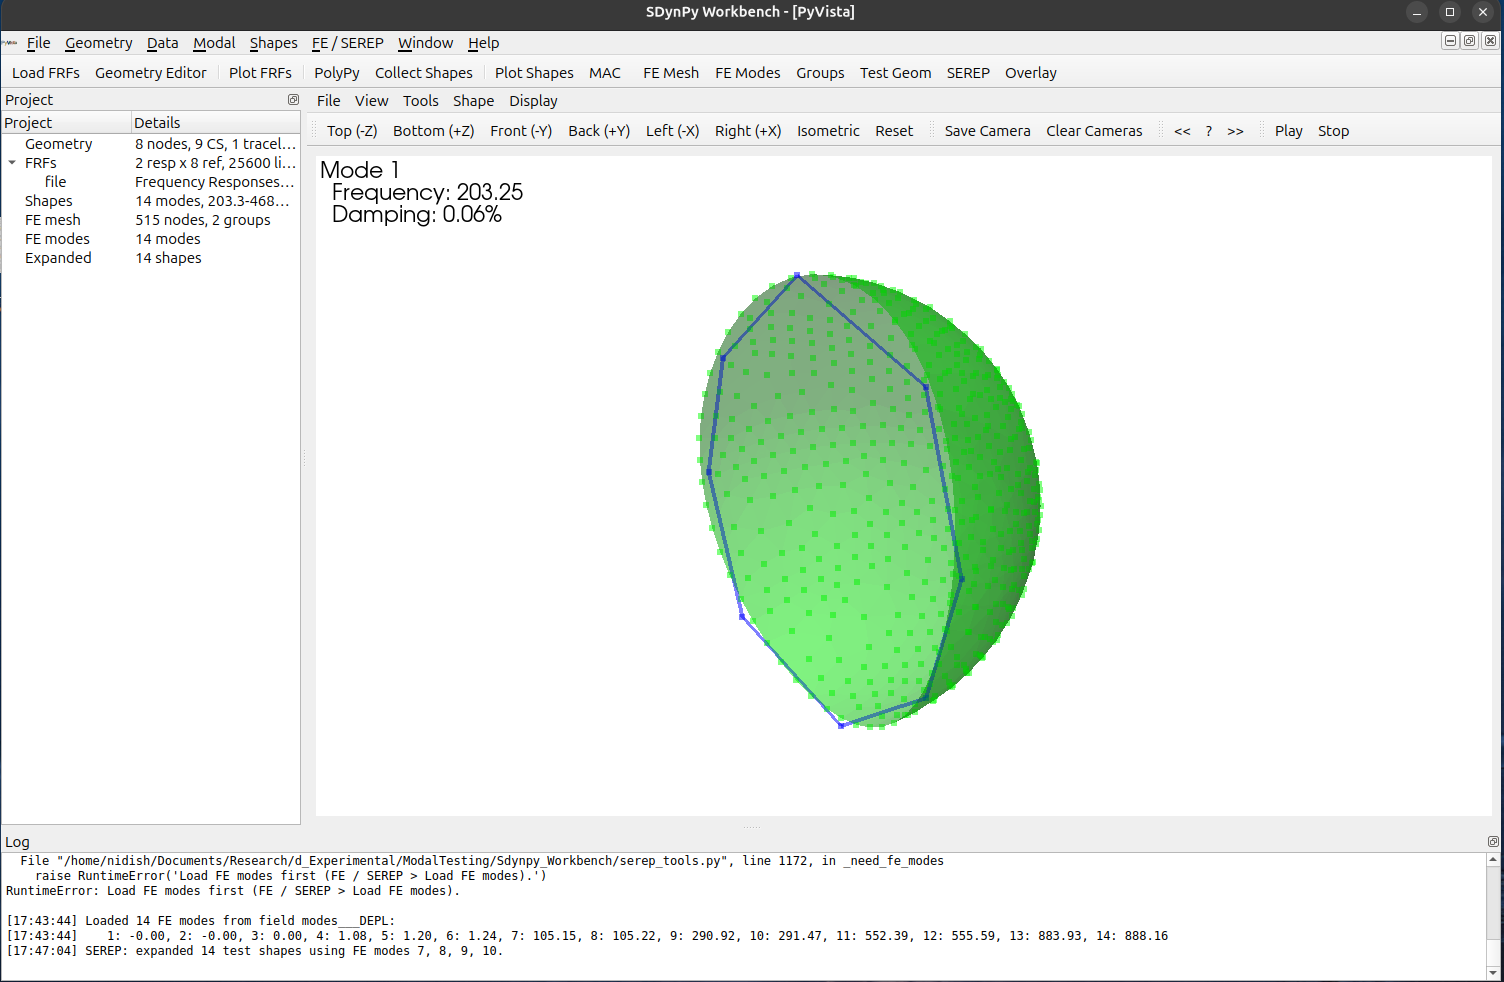
\includegraphics[width=.9\linewidth]{figs/overlay.png}
\caption{\label{fig:overlay}Test and Expanded shapes overlaid. GUI state after clicking on \texttt{Overlay}}
\end{figure}
\section{Inspect the Modal Assurance Criterion.}
\label{sec:org620c196}

You can do other things like the test-model MAC visualization by clicking on \texttt{FE/SEREP->Plot MAC:expanded vs FE modes}. \Cref{fig:mac} shows this for the current example.

\begin{figure}[!h]
\centering
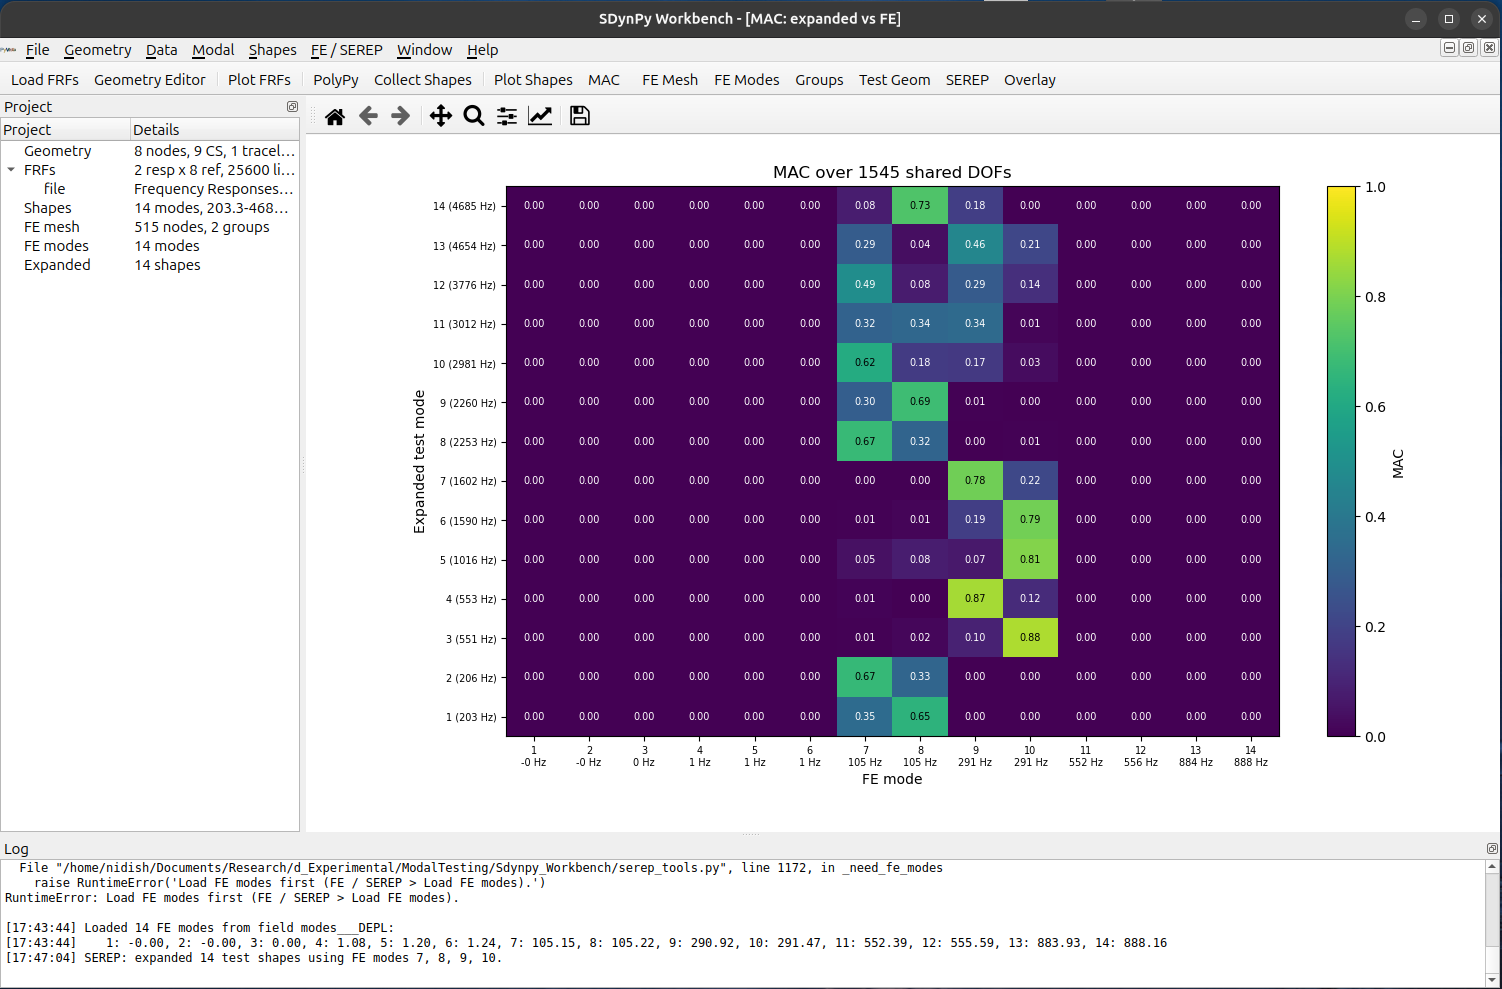
\includegraphics[width=0.75\textwidth]{figs/mac.png}
\caption{\label{fig:mac}Expanded Test vs FE mode MACs.}
\end{figure}
\section{Saving the work/Loading historical work}
\label{sec:org65d593c}

The complete session (except for the PolyPy internals) can be saved through \texttt{File->Save Workbench}. This can be helpful to continue from where on leaves off later.
\end{document}
